\section{Inledning}
Jag ska göra en filhanterar som visar alla filer och mappar i 3D. Det finns många tidigare exempel på liknande projekt såsom File System Navigator(FSN) som man kan se i filmen Jurassic park, se figur~\ref{fig:fsn}. Ett nyare exempel är TDFSB som också visar bilder i alla mappar, kan spela upp ljud och film samt är alla mappar portaler som transporterar en till den nya mappen, se figure~\ref{fig:tdfsb}:
\begin{center}
\begin{figure}[H]
    \centering
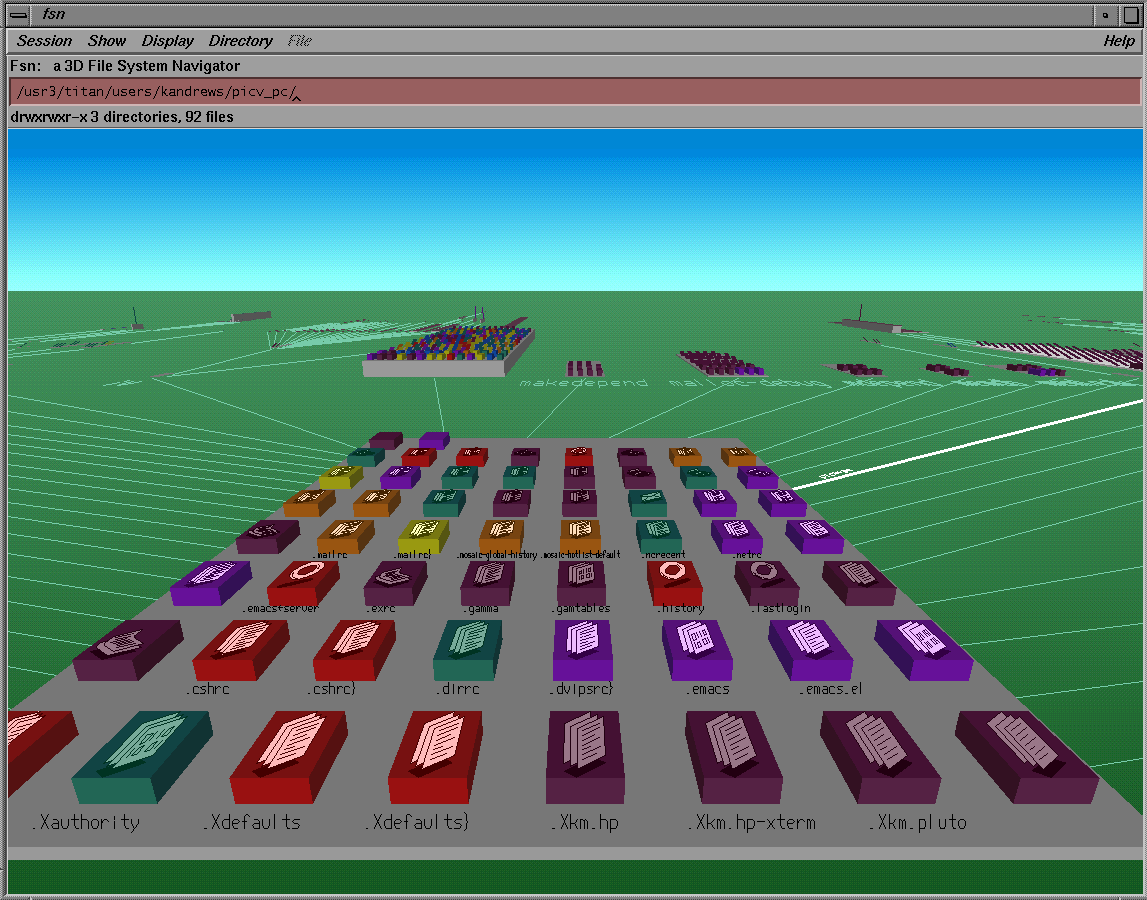
\includegraphics[width=6cm]{../grafik/fsn1.png}
\caption{FSN.}
\label{fig:fsn}
\end{figure}
\end{center}

\begin{center}
\begin{figure}[H]
    \centering
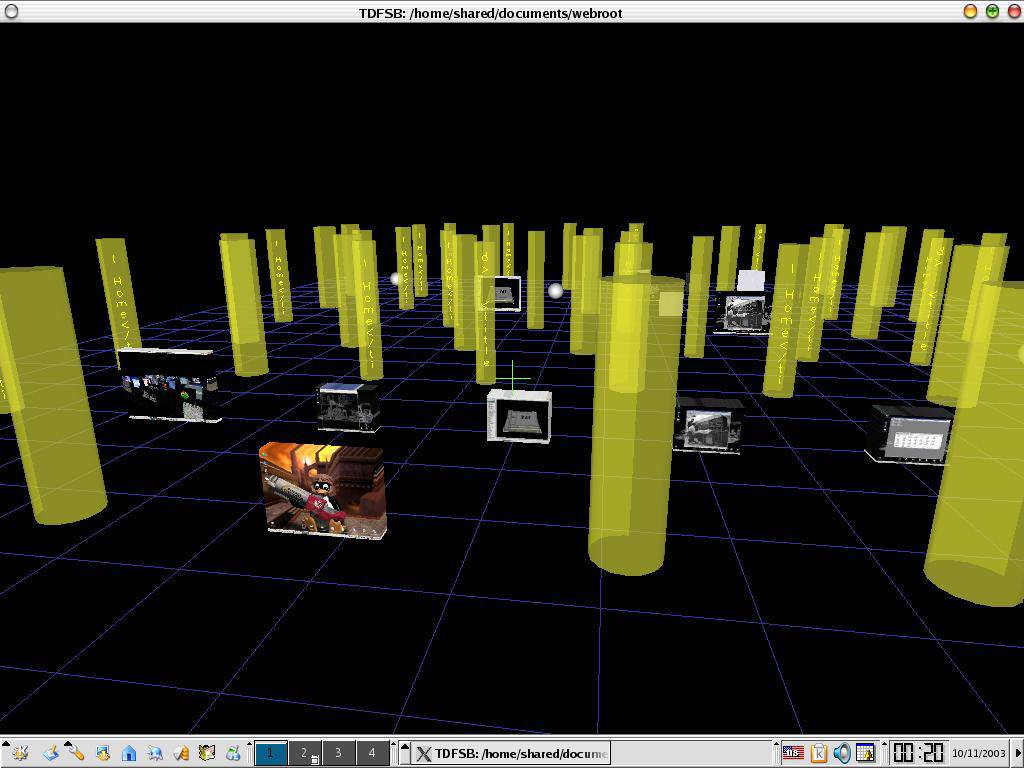
\includegraphics[width=6cm]{../grafik/tdfsb.jpg}
\caption{TDFSB.}
\label{fig:tdfsb}
\end{figure}
\end{center}